\documentclass[border=3pt,tikz]{standalone}
\usepackage[utf8]{vietnam}
\usetikzlibrary{calc,angles,intersections,shapes.geometric,arrows,decorations.markings,arrows.meta,patterns.meta,patterns}
\usepackage{tikz-3dplot,pgfplots}
\pgfplotsset{compat=1.15}
\usepgfplotslibrary{polar}
\usepackage{amsmath}
\begin{document}
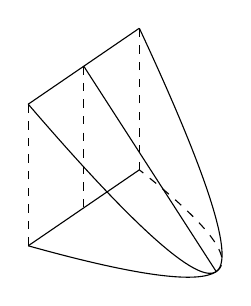
\begin{tikzpicture}
	\begin{axis}
		[axis x line=middle,axis y line=middle,axis z line=middle,axis equal,no markers,minor tick num=0,hide axis,view={-50}{35}]
		\addplot3[black,samples=300,samples y=0,domain=-2:0,variable=t] (t, t^2, 0);
		\addplot3[black,samples=300,samples y=0,dashed,domain=0:2,variable=t] (t, t^2, 0);
		\addplot3[black,samples=300,samples y=0,variable=t,domain=-2:2] (t, t^2, t^2);
		\addplot3[black] coordinates {(-2,4,0)(2,4,0)};
		\addplot3[black] coordinates {(-2,4,4)(2,4,4)};
		\addplot3[black] coordinates {(0,0,0)(0,4,4)};
		\addplot3[black,dashed] coordinates {(0,4,4)(0,4,0)};
		\addplot3[black,dashed] coordinates {(2,4,0)(2,4,4)};
		\addplot3[dashed] coordinates {(-2,4,0)(-2,4,4)};
	\end{axis}
\end{tikzpicture}
\end{document}
